\documentclass[11pt]{article}




\usepackage{fancyhdr}
\usepackage{amsthm}
\usepackage{amssymb}
\usepackage{amsmath}
\usepackage{setspace}
\usepackage{graphicx}
\usepackage{enumitem}
\setenumerate[1]{label=(\alph*)}

\pagestyle{fancyplain}



\newtheorem{theorem}{Theorem}[section]
\newtheorem*{theorem*}{Theorem}
\newtheorem{lemma}[theorem]{Lemma}
\newtheorem{proposition}[theorem]{Proposition}
\newtheorem{corollary}[theorem]{Corollary}
\newtheorem{definition}{Definition}
\begin{document}

\lhead{Frederick Robinson}
\rhead{Math 410-3: Complex Analysis}



\title{Final Exam}
\author{Frederick Robinson}
\date{5 June 2011}
\maketitle

$D(a,r)$ is the disc of radius $r$ centered at $a$.

\section{Problem 1}\label{problem1}
\subsection{Question}
Let 
\[p_N = z^N + a_{N-1} z^{N-1} + \cdots  + a_0\]
be a monic polynomial of degree $N$ and consider the function $|p_N(z)|^2$ on $\mathbb{C}$. The following is a sequence of questions about the critical points and level curves $\{ z \ :\  |p_N (z)|^2 = t\}$ for the polynomial. In each case, prove that your answer is correct. Note that the leading coefficient equals 1 (i.e. $p_N$ is monic).
\begin{enumerate}  
\item Exactly how many local minima does $|p_N(z)|^2$ have on $\mathbb{C}$?
\item Exactly how many local maxima does it have?
\item Exactly how many saddle points?
\item For each $t \in (0 , \infty)$, what is the maximum number of connected components of the ``level curve" $\{z \ : \ |p_N(z)|^2=t\}$?
\item \label{lastprob} Show that $M(r) = \sup_{|z| =r} |p_N(z)|^2$ is increasing with $r$.
\item Show that $m(r) = r^{-2N} \sup_{|z|=r} |p_N(z)|^2$ is decreasing with $r$. [\emph{Hint:} $z^N p_N( \frac{1}{z})$ is also a polynomial of degree $N$.]
\end{enumerate} 
\subsection{Answer}
Assume throughout that $p_N$ is nonconstant.
\begin{enumerate}
\item The function $|p_N(z)|^2$ has as many local minima as $p_N(z)$ has distinct zeros. 
\begin{proof}
If $a$ is a zero of $p_N$ then it is a local minimum of $|p_N|^2$, since $|p_N|^2$ has only finitely many zeros, and is nonnegative. Conversely, if $a$ is a local minimum of $|p_N|^2$ it is a local minimum of  $|p_N(a)|$ and must therefore have $|p_N(a)| = |p_N(a)|^2 = 0 $ by the minimum modulus principle (apply the maximum modulus principle to $1/z$).
\end{proof}
\item By the maximum modulus principle (Theorem 5.4.2) there are no local maxima of $|p_N|$, and there may therefore by no local maxima of $|p_N|^2$.
\item Denote $p_N = u + i v$, and assume $a$ is a critical point of $|p_N|^2$. Then, by definition 
\begin{align}
\label{trivial} \frac{\partial}{\partial x} \left( u^2 + v^2 \right) &= 0\\
2 u \frac{\partial u}{\partial x}  + 2 v \frac{\partial v }{\partial x} &= 0.
\end{align}
Similarly, 
\begin{align}\label{magic}2u \frac{\partial u}{\partial y} + 2 v \frac{\partial v}{\partial y} = 0. \end{align}
Then, applying the Cauchy Riemann equations to  (\ref{magic}), we have
\[2 u \frac{\partial v}{\partial x} =  2 v \frac{\partial u }{\partial x}.\]
Combining this, with (\ref{trivial}) we have
\[- v^2 \frac{\partial v}{\partial x} = u^2 \frac{\partial v}{\partial x} \quad\mbox{and}\quad - u^2 \frac{\partial u}{\partial x} = v^2 \frac{\partial u}{\partial x} \]
or equivalently, 
\[ (u^2+ v^2) \frac{\partial v}{\partial x}  = 0 \quad\mbox{and}\quad ( u^2 + v^2) \frac{\partial u}{\partial x} = 0 \]
However, if $u^2 + v^2 =0$ at some point it must  be a local minimum. Therefore, every saddle point has $\partial v/ \partial x = \partial u / \partial x = 0$ (i.e. $\partial / \partial z = 0) $. 

So, saddle points are all $a$ with  $\partial f / \partial z ( a) = 0$ which do not have also $f(a) = 0$. This is bounded above by the number of roots of $f$ less one, as multiple roots of $f$ are also roots of $\partial f \partial z$ with multiplicity one less than their multiplicity in $f$.
\item 
Denote 
\[A = \{ f(a) \mid \frac{\partial f }{ \partial z}( a ) = 0, f(a) \neq 0\}\]
where $f(a)$ appears $n$ times if $n$ is the multiplicity of the root $a$ of $\partial f / \partial z$. This is the set of saddle points with multiplicity. If we denote also
\[C(x) = |\{ b \mid b \in A , b > x\} | \]
then the number of connected components of $L_t$ is just $C(t) + 1$.

\begin{proof}
The number of connected components of the level curve $L_t = \{z \ : \ |p_N(z)|^2=t\} $ is the same as the number of local minima for some sufficiently small $t$ by definition of local minimum, together with the fact that all local minima have $f(m) =0$. 

As we increase $t$ the connected components grow, getting closer together until  they reach a member of $A$, where they are tangent at the saddle point. If the saddle point is a multiple root, then more than one connected component is tangent at the same point corresponding to the multiplicity of the root. 
\end{proof}
\item 
\begin{proof}
Suppose towards a contradiction that $M$ is not increasing with $r$. Then, by continuity, there exist $r, \epsilon >0$ such that for every $r' < r + \epsilon, M(r') \leq M(r)$. Fix such $r, \epsilon$, and fix $x$ such that $|x| = r, M(r) = f(x)$.

We must have $f'(x) = 0$ as if $f'(x)  \neq 0$, then $f'(x) $ is normal to the circle, and pointing outwards (as $f(x)$ is assumed to be maximal on the circle).  Thus, an arbitrarily small increase in the size of the circle will increase the value of $M$, choosing $|x'| = r + \epsilon$ as $x' = (1+\epsilon/r) (x)$.

So, $x$ is a saddle point, or a local minimum. If it's a local minimum we have the desired contradiction, so assume that it's a saddle point. This too is contradictory however. There is a direction in which the second derivative is positive. If this is tangent to the circle, then $x$ was not a maximal choice, and if it is not, then we may move in this direction to find an $x'$ with $f(x')> f(x)$.
\end{proof}
\item Per the hint observe that $z^N p_N(\frac{1}{z})$ is a polynomial of degree $N$, and so by the previous part, the following is increasing in $r$
\[\sup_{|z| =r} \left|z^N p_N\left(\frac{1}{z}\right)\right|^2 = r^{2N} \sup_{|z| =r}\left| p_N\left(\frac{1}{z}\right)\right|^2 \]
Thus, substituting $z = 1/z$ we have that 
\[ r^{-2N} \sup_{|z| =r} \left| p_N\left(z\right)\right|^2 \]
is decreasing in $r$, as desired.
\end{enumerate}


\section{Problem 2}
\subsection{Question}
Let $P(z) = z^n + a_{n-1} z^{n-1} + \cdots + a_1 z+ a_0$ be a monic polynomial of degree $n \geq 2$. Let $C$ be the boundary of a disc containing all of the zeros of $P(z)$. Evaluate the following integrals:
\begin{enumerate}
\item \[\int_C \frac{dz}{P(z)} . \]
\item \[ \int_C \frac{z P'}{P} dz .\]
\end{enumerate}
\subsection{Answer}
\begin{enumerate}
\item We can apply the Residue theorem, to obtain
\[2 \pi i \sum_{j=1}^m  \mbox{Res}_f(p_j)\]
since the winding number about any pole is just 1. More specifically, if we write
\[P(z) = (z - p_1) ^{k_1} (z - p_2)^{k_2} \cdots (z-p_m)^{k_m}\]
that is
\begin{align*}
\int_C \frac{dz}{P(z)}  &= 2 \pi i \sum_{j=1}^m  \mbox{Res}_f(p_j)\\
&= 2 \pi i \sum_{j=1}^ m\frac{1}{(k_j-1)!} \left. \left( \frac{\partial}{\partial z}\right) ^{k_j-1} \left( ( z-p_j)^{k_j} f(z)\right) \right|_{z=p_j}
\end{align*}
\item
We can apply the Residue theorem, to obtain
\[2 \pi i \sum_{j=1}^m  \mbox{Res}_f(p_j)\]
since the winding number about any pole is just 1.
Some manipulation reveals that this is just
\[ \sum_{j=1}^m k_j p_j.\]
\end{enumerate}


\section{Problem 3}
\subsection{Question}
Does there exist a holomorphic function $f: D(0,1) \to D(0,1)$ such that $f(0) = \frac{1}{2}$ and such that $f'(0) = \frac{4}{5}$? Prove that your answer is correct.
\subsection{Answer}
No.
\begin{proof}
Assume that $f: D(0,1) \to D(0,1)$ is holomorphic with $f(0) = \frac{1}{2}$.  By the  Schwarz-Pick theorem, 
\[f'(0) \leq 1 - \left|\frac{1}{2}\right|^2 = \frac{3}{4}\]
\end{proof}

\section{Problem 4}
\subsection{Question}
Let $p(z;t) = z^n + a_{n-1} (t) z^{n-1} + \cdots + a_1(t) z  + a_0(t)$ be a family of polynomials of degree $n$ with $a_j(t)$ continuous in the real parameter $t \in [0,1]$. Suppose that $p(z;0)$ has $k$ zeros in the disc $|z-a| < r$ and no zeros on the circle $|z-a| = r$. 
\begin{enumerate}
\item Show that for sufficiently small $t, p(z;t)$ has $k$ zeros in $|z-a| <r$.
\item Show that the zeros of $p(z;t)$ are continuous in $t$.
\end{enumerate}
\subsection{Answer}
\begin{enumerate}
\item This is a consequence of Rouch\'{e}'s Theorem.  If we denote $f = p(z;0), g = z; \epsilon)$, then for some $\epsilon > 0$, for each $\zeta$ in the boundary of our disk, we have 
\[|f(\zeta) - g(\zeta)| < |g(\zeta)|,\]
by continuity of the $a_j$ and since there are no zeros in the boundary.
\item We need to show that if $p(z;t_0)$ has zero at $p_0$, given $\delta > 0 $, there is $\epsilon$, such that  the zeros of $f(z; D(t_0,\epsilon)) $ are in $  D(p_0, \delta)$.  

This follows directly from the first part, if we take $ a = \delta$.
\end{enumerate}

\section{Problem 5}
\subsection{Question}
Let $c> 0$, $a>0\in \mathbb{R} $. Use the residue calculus to evaluate the integrals
\[\psi(z) : = \int_{\Re z =c} \frac{a^z}{z^2} dz\]
\subsection{Answer}We will integrate around the contour pictured below, say $\gamma_r$ where $\alpha_r$ is the left portion of the circle of radius $r$ centered at 0.
\begin{center}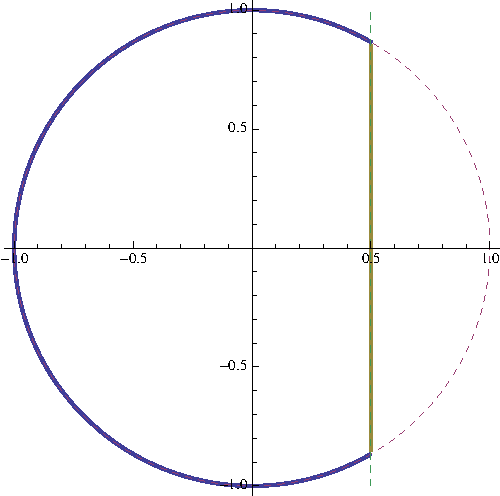
\includegraphics[width=60mm]{contour.pdf}\end{center}
\[\int_{\gamma_r} \psi(z) = \int_{\stackrel{\Re z = c}{|z|\leq r}} \psi(z) + \int_{\alpha_r} \psi(z).\]  
Observe that 
\begin{align*} \left| \int_{\alpha_r} \psi(z) \right| & \leq |\alpha_r| \cdot | \sup_{\alpha_r} \psi(z)|\\
& \leq |\alpha_r| \cdot | \frac{a^c}{r^2}|\\
& \leq r | \frac{a^c}{r^2}|\\
&= | \frac{a^c}{r}|
\end{align*}
where $|\alpha_r|$ denotes the length of $\alpha_r$.

Therefore, as $ r \to \infty$ 
\[  \int_{\stackrel{\Re z = c}{|z|\leq r}} \psi(z) \to \int_{\gamma_r} \psi(z) .\]  
and by the residue theorem 
\[ \int_{\gamma_r} \psi(z) =\left. 2 \pi i \frac{\partial}{\partial z} a^z \right|_{z=0} =2 \pi \log{a} =  \int_{\Re z = c} \psi(z) .\]

\section{Problem 6}
\subsection{Question}
Find all entire holomorphic functions $f$ on $\mathbb{C}$ such that $ |f(z)| \geq 1$ for all $z$. 
\subsection{Answer}
Clearly, any constant value $f(z) = c$ with $|c| \geq 1$ fulfills the requirements. This is the only possibility.
\begin{proof}
Suppose that $f $ is a finite (nonconstant) polynomial. Then it has zeros, and so cannot have the desired property. 

The only other possibility is that $f$ be nonpolynomial. However, by examining the Laurent series of $f(1/z)$ we see that this  implies $f$ has an essential singularity at $\infty$, and so the function applied to some neighborhood of $\infty$ is dense in $\mathbb{C}$ a contradiction.
\end{proof}


\section{Problem 7}
\subsection{Question}
Let $U$ be a bounded holomorphically simply connected domain. Let $a \in U$. Suppose that $f: U \to U$ is a holomorphic function  such that $f(a) = a$, $|f'(a)| = 1$. Show that $f$ is 1-1 and onto. 
\subsection{Answer}
\begin{proof}
By Schwarz's Lemma $f$ is a rotation about $a$. Thus, $f$ must be injective. 

The map $f^{-1}: f(U) \to U$ (the rotation backwards by the same amount as $f$) is  well defined as $f$ is injective, and an injection being itself a rotation. Hence, $f$ is bijective, as desired.
\end{proof}


\section{Problem 8}
\subsection{Question}
Let $f(z) = \sum_{n=0}^\infty a_n z^n$ be an entire function.
\begin{enumerate}
\item State the most general Cauchy estimates for $|\frac{d^k}{dz^k} f(0)|$.
\item Suppose that 
\[|f(z)| \leq Ce^{c|z| ^\rho}.\]
Show that
\begin{align} \label{result} \limsup_{n \to \infty} |a_n| ^{1/n} n^{\frac{1}{\rho}}< \infty.\end{align}
\item Conversely, suppose that (\ref{result}) holds. Show that for all $\epsilon > 0$, $|f(z) | \leq Ce^{c|z|^{\rho + \epsilon}}$.
\end{enumerate}
\subsection{Answer}
\begin{enumerate}
\item \[ \left|\frac{d^k}{dz^k} f(0)\right| \leq \frac{M k!}{r^k}\]
for $M = \sup_{z \in \overline{D}(0,r)} |f(z)|$, $r > 0$.
\item Since
\[a_k = \frac{1}{k!} \left| \frac{d^k}{dz^k} f(0) \right| ,\]
Cauchy estimates imply that
\[a_k \leq \frac{M}{r^k}.\]
Thus, 
\begin{align*}
|a_n|^{1/n} n^{\frac{1}{\rho}} &\leq \left| \frac{M}{r^n} \right|^{1/n} n^{\frac{1}{\rho}}    \\
&=  \left| \frac{M^{1/n}}{r} \right| n^{\frac{1}{\rho}}     \\
&\leq   \left| \frac{(Ce^{c|z|^\rho})^{1/n}}{z} \right| n^{\frac{1}{\rho}}     \\
\end{align*}
Choosing $|z| = n^{1/\rho}$ this is
\[ |a_n|^{1/n} n^{\frac{1}{\rho}} \leq  \left| Ce^c \right|  \]
As this bound is not dependent on $n$, we have the desired result.
\item Suppose
\[\limsup_{n \to \infty} |a_n|^{1/n} n ^{1/ \rho} = C < \infty.\]
Then, for all $\epsilon > 0$ there exists $N$ such that for all $n >N$
\[|a_n|^{1/n} n ^{1/\rho} < C + \epsilon.\]
Rewriting, we have
\[|a_n| < \left( \frac{(C+ \epsilon)^\rho}{n}\right)^n\]
for sufficiently large $n$. Thus, 
\[ |f(z)|  = \sum_{i=0}^\infty |a_i| |z|^i < K\left(\sum_{i=0}^\infty \left( \frac{(C+ \epsilon)^\rho}{i}\right)^i  |z|^i \right)\]
where the $K$ is introduced to take care of the first (finitely many) terms until the inequality holds. Now, observe
\begin{align*}
 |f(z)|  & < K\sum_{i=0}^\infty \left( \frac{(C+ \epsilon)^\rho}{i} |z|\right)^i  \\ 
&< K\sum_{i=0}^\infty  \frac{1}{i !}((C+ \epsilon)^\rho |z|)^i  \\
& = K e^{(C+ \epsilon)^\rho |z|}.
\end{align*}
After a relabeling of constants, we have 
\[|f(z) | \leq Ce^{c|z|^{\rho + \epsilon}}\]
as desired.
\end{enumerate}

\section{Problem 9}
\subsection{Question}
Let $\{ f_n\}$ be a uniformly bounded family of holomorphic functions in an open set $U \subset \mathbb{C}$. Suppose that there exists a subset $E \subset U$ which has an accumulation point in $U$ such that $\lim_{n \to \infty} f_n(w) $ exists for all $w \in E$.
\begin{enumerate}
\item Prove that $f_n$ converges uniformly on compact subsets $K \subset U$ to a holomorphic function $f$.
\item How is the conclusion stronger than that of Montel's theorem?
\end{enumerate}
\subsection{Answer}
\begin{enumerate}
\item By Montel's theorem, there is some subsequence $\{f_m\} \subseteq \{f_n\}$ which converges normally on $U$ to a limit holomorphic function $f$. Since $\lim_{n \to \infty} f_n(w)$ exists for each $w \in E$, we know that the whole sequence converges, not just the subsequence:
\[\lim_{n \to \infty} f_n(w) = f(w).\]
However, since $E$ has a limit point, this generalizes to the entire domain $U$ (3.6.3) and 
\[ \lim_{n \to \infty} f_n(x) = f(x)\]
without restriction.
\item This is stronger than Montel's theorem since it gives us a particular sequence which converges, not just convergent subsequences.

\end{enumerate}


\section{Problem 10}
\subsection{Question}
Consider the following `functional' on the space $\mathcal{P}_N$ of monic polynomials of degree $N$:
\[M(P) = \sup_{|z| = 1} |P(z)|.\]

Find the polynomial $P$ which \emph{minimizes} $M$, i.e. with the minimum value of $M(P)$. Prove that your answer is correct.
\subsection{Answer}
The desired polynomial is $f_n = z^n \in \mathcal{P}_N$.
\begin{proof}
Employing Cauchy Estimates on $D(0,1)$, we have 
\[\left| \frac{\partial^k f}{\partial z^k} (0) \right| \leq L k !\]
for $L = \sup_{z \in \overline{D}(0,1)} |f(z)|$. By \ref{problem1}\ref{lastprob} $\sup_{z \in |r|}|f(z)|$ is increasing in $r$. Thus, $L = M(P)$, and
\[ \frac{1}{k!} \left| \frac{\partial^k f}{\partial z^k} (0) \right| \leq M(P) .\]
For $f$ a monic polynomial of degree $k$, we then have
\[M(P) \geq 1.\]
This bound is tight for the polynomial $f_n = z^n \in \mathcal{P}_N$.\end{proof}



\end{document}
